\documentclass[conference]{IEEEtran}
\IEEEoverridecommandlockouts
% The preceding line is only needed to identify funding in the first footnote. If that is unneeded, please comment it out.
\usepackage{cite}
\usepackage{amsmath,amssymb,amsfonts}
\usepackage{algorithmic}
\usepackage{graphicx}
\usepackage{url}
\usepackage[utf8]{inputenc}
\usepackage{textcomp}
\usepackage{multirow}
\usepackage{booktabs}
\usepackage{subfig}
\usepackage{nameref}

\usepackage[english]{babel}
\DeclareUnicodeCharacter{00A0}{ }
\def\BibTeX{{\rm B\kern-.05em{\sc i\kern-.025em b}\kern-.08em
    T\kern-.1667em\lower.7ex\hbox{E}\kern-.125emX}}
\begin{document}

\title{Skin Lesion Segmentation and Classification --\\
  UnB entry at the ISIC Challenge}

\author{\IEEEauthorblockN{Frederico Guth\IEEEauthorrefmark{1},
Teófilo E. de Campos \IEEEauthorrefmark{2}}
\IEEEauthorblockA{Departamento de Ciência da Computação,
Universidade de Brasília (UNB)\\
\IEEEauthorrefmark{1}fredguth@fredguth.com,
\IEEEauthorrefmark{2}t.decampos@st-annes.oxon.org}}

\maketitle


\begin{abstract}
  This paper describes our approach for the ISIC Challenge 2018 - Skin Lesion Analysis Towards Melanoma Detection. For Part 1 - Lesion Segmentation, we developed a U-Net based convolutional neural network pretrained with the ImageNet dataset and applied several data augmentation and hyperparameters optimization strategies, obtaining threshold Jaccard index of 77.5\%. For Part 3 - Lesion Classification, we developed an ensemble strategy that achieved an online score of 84.6\%. 
\end{abstract}

\section{Introduction}

According to the World Health Organization, between 2 and 3 million non-melanoma skin cancers and 132,000 melanoma skin cancers occur globally each year \cite{who}. Despite representing less than 6.5\% of all skin cancers, melanomas are the most dangerous type, accounting for aproximately 75\% of all skin cancer related deaths \cite{who,nature}.
Early detection is critical to increase survival expectancy and visual inspection still is the most common diagnostic technique.

Deep convolutional neural networks (CNNs) already exceed human performance in visual classification\cite{fei}.
In some areas of oncology, such as histological image analysis, CNNs have also proven to match the performance of experts, e.g.\ \cite{veta_etal_mia2015}.
In an attempt to improve the scalability of diagnostic expertise, CNNs have been developed to locate and classify skin cancers in images with dermatologist-level accuracy \cite{nature}.

Dermoscopy is a technique for examination of skin lesions that, with proper training, increase dianostic accuracy from 60\% (unaided expert visual inspection) to 75\%-84\%\cite{isic}. The International Skin Imaging Collaboration (ISIC) has a large-scale publicly acessible dataset of more than 20,000 dermoscopy images and host an annual benchmark challenge on dermoscopic image analysis since 2016.  The challenge comprise 3 tasks of lesion analysis: Part 1 - Segmentation, Part 2 - Dermoscopic feature extraction, Part 3 - Classification. 

In this paper, we describe our approach for the ISIC Challenge 2018:
\begin{itemize}
\item \textbf{Section \ref{segmentation}} describes our methodology for \textbf{lesion segmentation};
\item \textbf{Section \ref{classification}} describes our methodology for \textbf{lesion classification};
\end{itemize}


\section{Lesion Segmentation}
\label{segmentation}


\subsection{Segmentation Model: Unet34}
Introduced in 2015, U-Net is an encoder-decoder architecture designed for biomedical image segmentation\cite{olaf}, with great results in image segmentation problems \cite{iglovikov}. In an U-Net, the output is an image with the same dimension of the input, but with one channel.  The encoder path is a typical CNN, where each downsampling step doubles the number of feature channels. But what makes this architecture unique is the decoder path, where each upsampling step input is a concatenation of the output of the previous step with the output of the corresponding (same height) downsampling step. This strategy enables precise localization with a very simple network. 

Resnet is a very successful architecture in several computer vision tasks \cite{he}. It mitigates the degradation problem that happens when very deep networks starts converging. Instead of learning a direct mapping $H(x) = y$, it learns the residual function  $F(x) = H(x)-x$, which can be reframed into $H(x) = F(x)+x = y$, where $F(x)$ is a stack of non-linear layers and $x$ is the identity function(input=output). The formulation of $F(x)+x$ can be implemented by feedforward neural networks with “shortcut connections”. Resnet34, specifically, is composed of an initial convolutional layer, 16 blocks of 2 layers and a final fully connected layer.

Unet34 is the idea of using a pretrained Resnet34 model as an U-Net encoder path \cite{fastai}. First, every step from the adaptive pooling onwards is removed, keeping only Resnet backbone. Then we save the output of results of the initial layer, 3rd , 8th, and 14th blocks (of 16 in total). During the upsampling we concatenate the output of those with the ouputs of upsampling steps. We used Adam optimizer and Binary Cross Entropy with Logits as the loss function.

\subsection{Data and Augmentation}
We used “ISIC 2018: Skin Lesion Analysis Towards Melanoma Detection” grand challenge datasets \cite{codella, ham} and no aditional external data. All images were first resized to 128x128 pixels, 256x256 and 512x512; and preprocessed to adjust color balance. Random transformations on input images to agument the dataset were made: dihedral transformation, rotation (up to 44 degrees), zooming (up to 1.05), fliping and random lightining changes. The official training dataset was then splited in 3-folds of training and validation datasets.  


\subsection{Segmentation Experiments and Training}
\label{sec:seg_training}
Our training strategy was to first train the model with 128x128 images and transfer this learning to train the same model with images with 256 x 256 images. We would suggest using the same strategy to go from 256x256 to 512 x 512 images, but due to GPU memory constraints, we did not manage to acccomplish this last step.

\begin{figure}
\centering
\subfloat[Learning Rate vs Validation Loss (Learning Rate Optimization)]{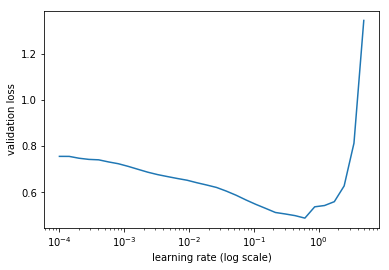
\includegraphics[width=.5\columnwidth]{LR_find.png}\label{lrfind}}
\subfloat[Iterations vs Learning Rate (cyclical learning rate policy)]{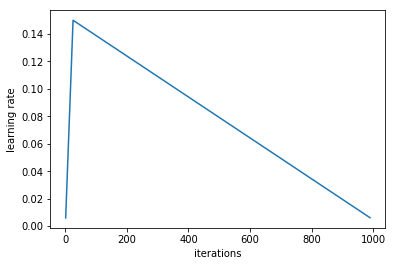
\includegraphics[width=.5\columnwidth]{lr_cycle.png}\label{sconv}}\hfil
\subfloat[Epoch vs Accuracy (superconvergence)]{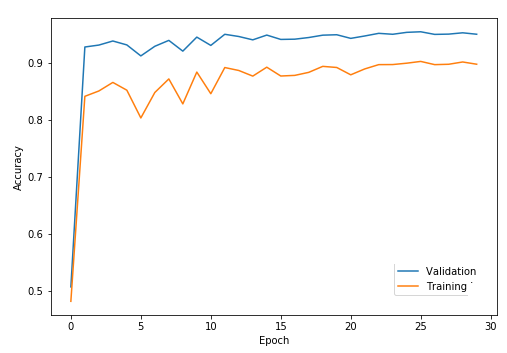
\includegraphics[width=0.6\columnwidth]{accuracy_epoch.png}}
\caption{Learning rate optimization strategy}\label{lr_find_chart}
\end{figure}

The training procedure was the same on 128x128 and 256x256:
\begin{enumerate}
  \item Freeze the first layer group.
  \item \label{lr_find}Define the optimal learning rate with the method proposed by \cite{leslie} and implemented by \cite{fastai}, where one batch is trained with different learning rates, starting at very low and linearly increasing it at every iteration and ploting a chart of the learning rate versus loss (see figure \ref{lrfind}).
  \item \label{superconvergence}We use the 1 cyclical learning rate policy (figure \ref{sconv}), also proposed by \cite{leslie}, to obtain training convergence in only 30 epochs (superconvergence).
  \item Unfreeze the model, keeping only the batch normalization layers frozen, and repeat steps \ref{lr_find} and \ref{superconvergence}.
\end{enumerate}

It would be advisable to use a loss function more similar to the avaliation criteria. As jaccard is not differentiable, one could use a soft jaccard variation\cite{iglovikov}. However, in our priliminar trials the implemented soft jaccard did not improve over the Binary Cross Entropy with Logits loss function and we decided to keep the later. 

We developed two strategies for Task 1:
\emph{BestDice}: This strategy just predicts the input with the model that presented the best dice index on the validation of our splited training dataset. 
\emph{Ensemble}: We used the 3-folds of our training dataset and trained with BestDice model and ensemble than to give a prediction. 

\subsection{Segmentation Results}

\begin{figure}
\centering
\subfloat[Good Result Sample\label{good}]{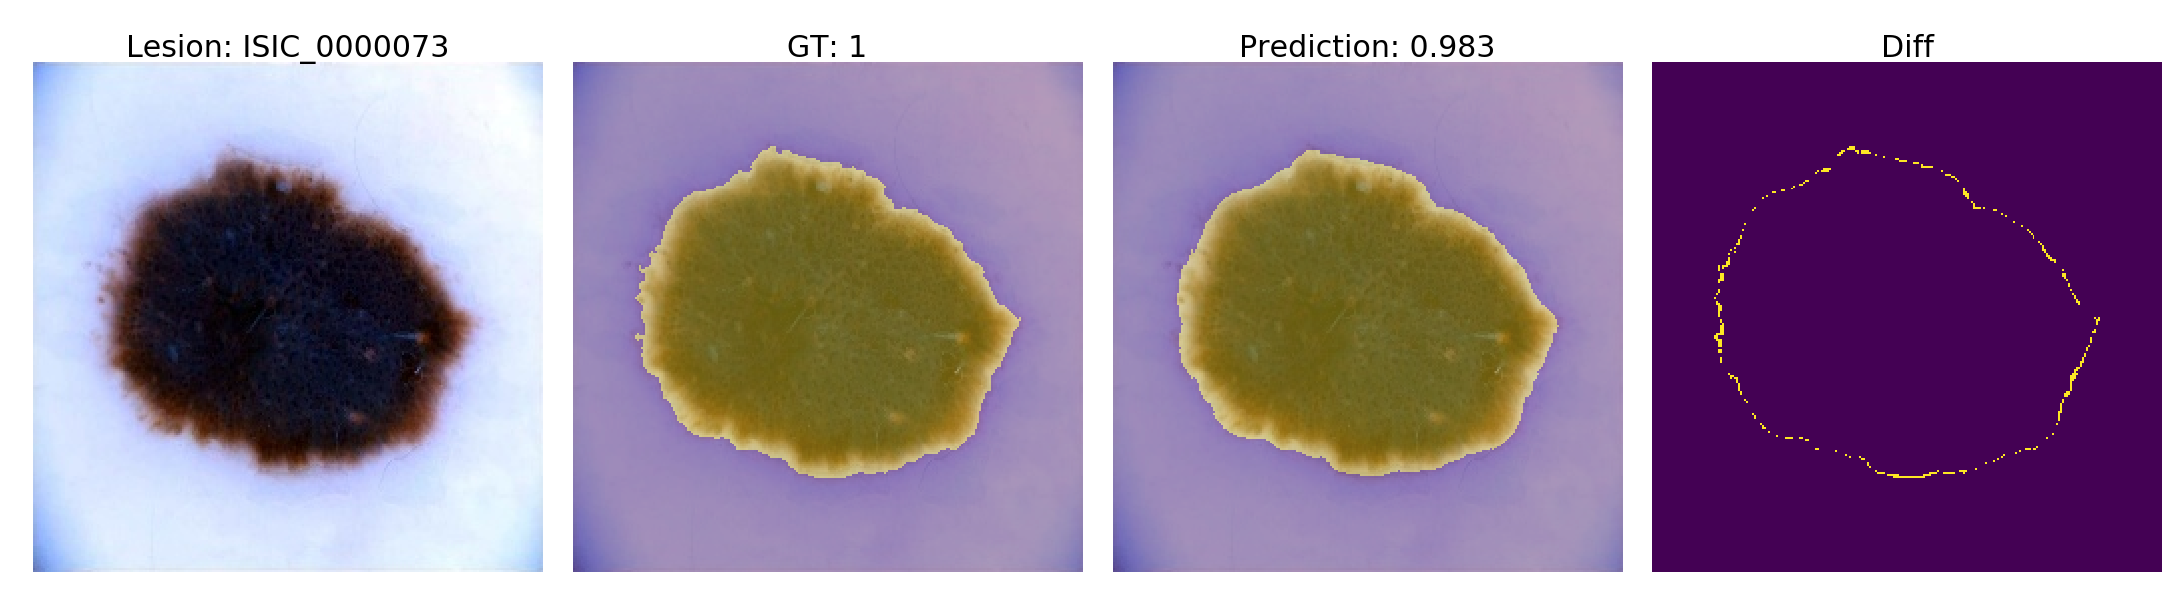
\includegraphics[width=\columnwidth]{good_result.png}}\hfil
\subfloat[Bad Result Samples]{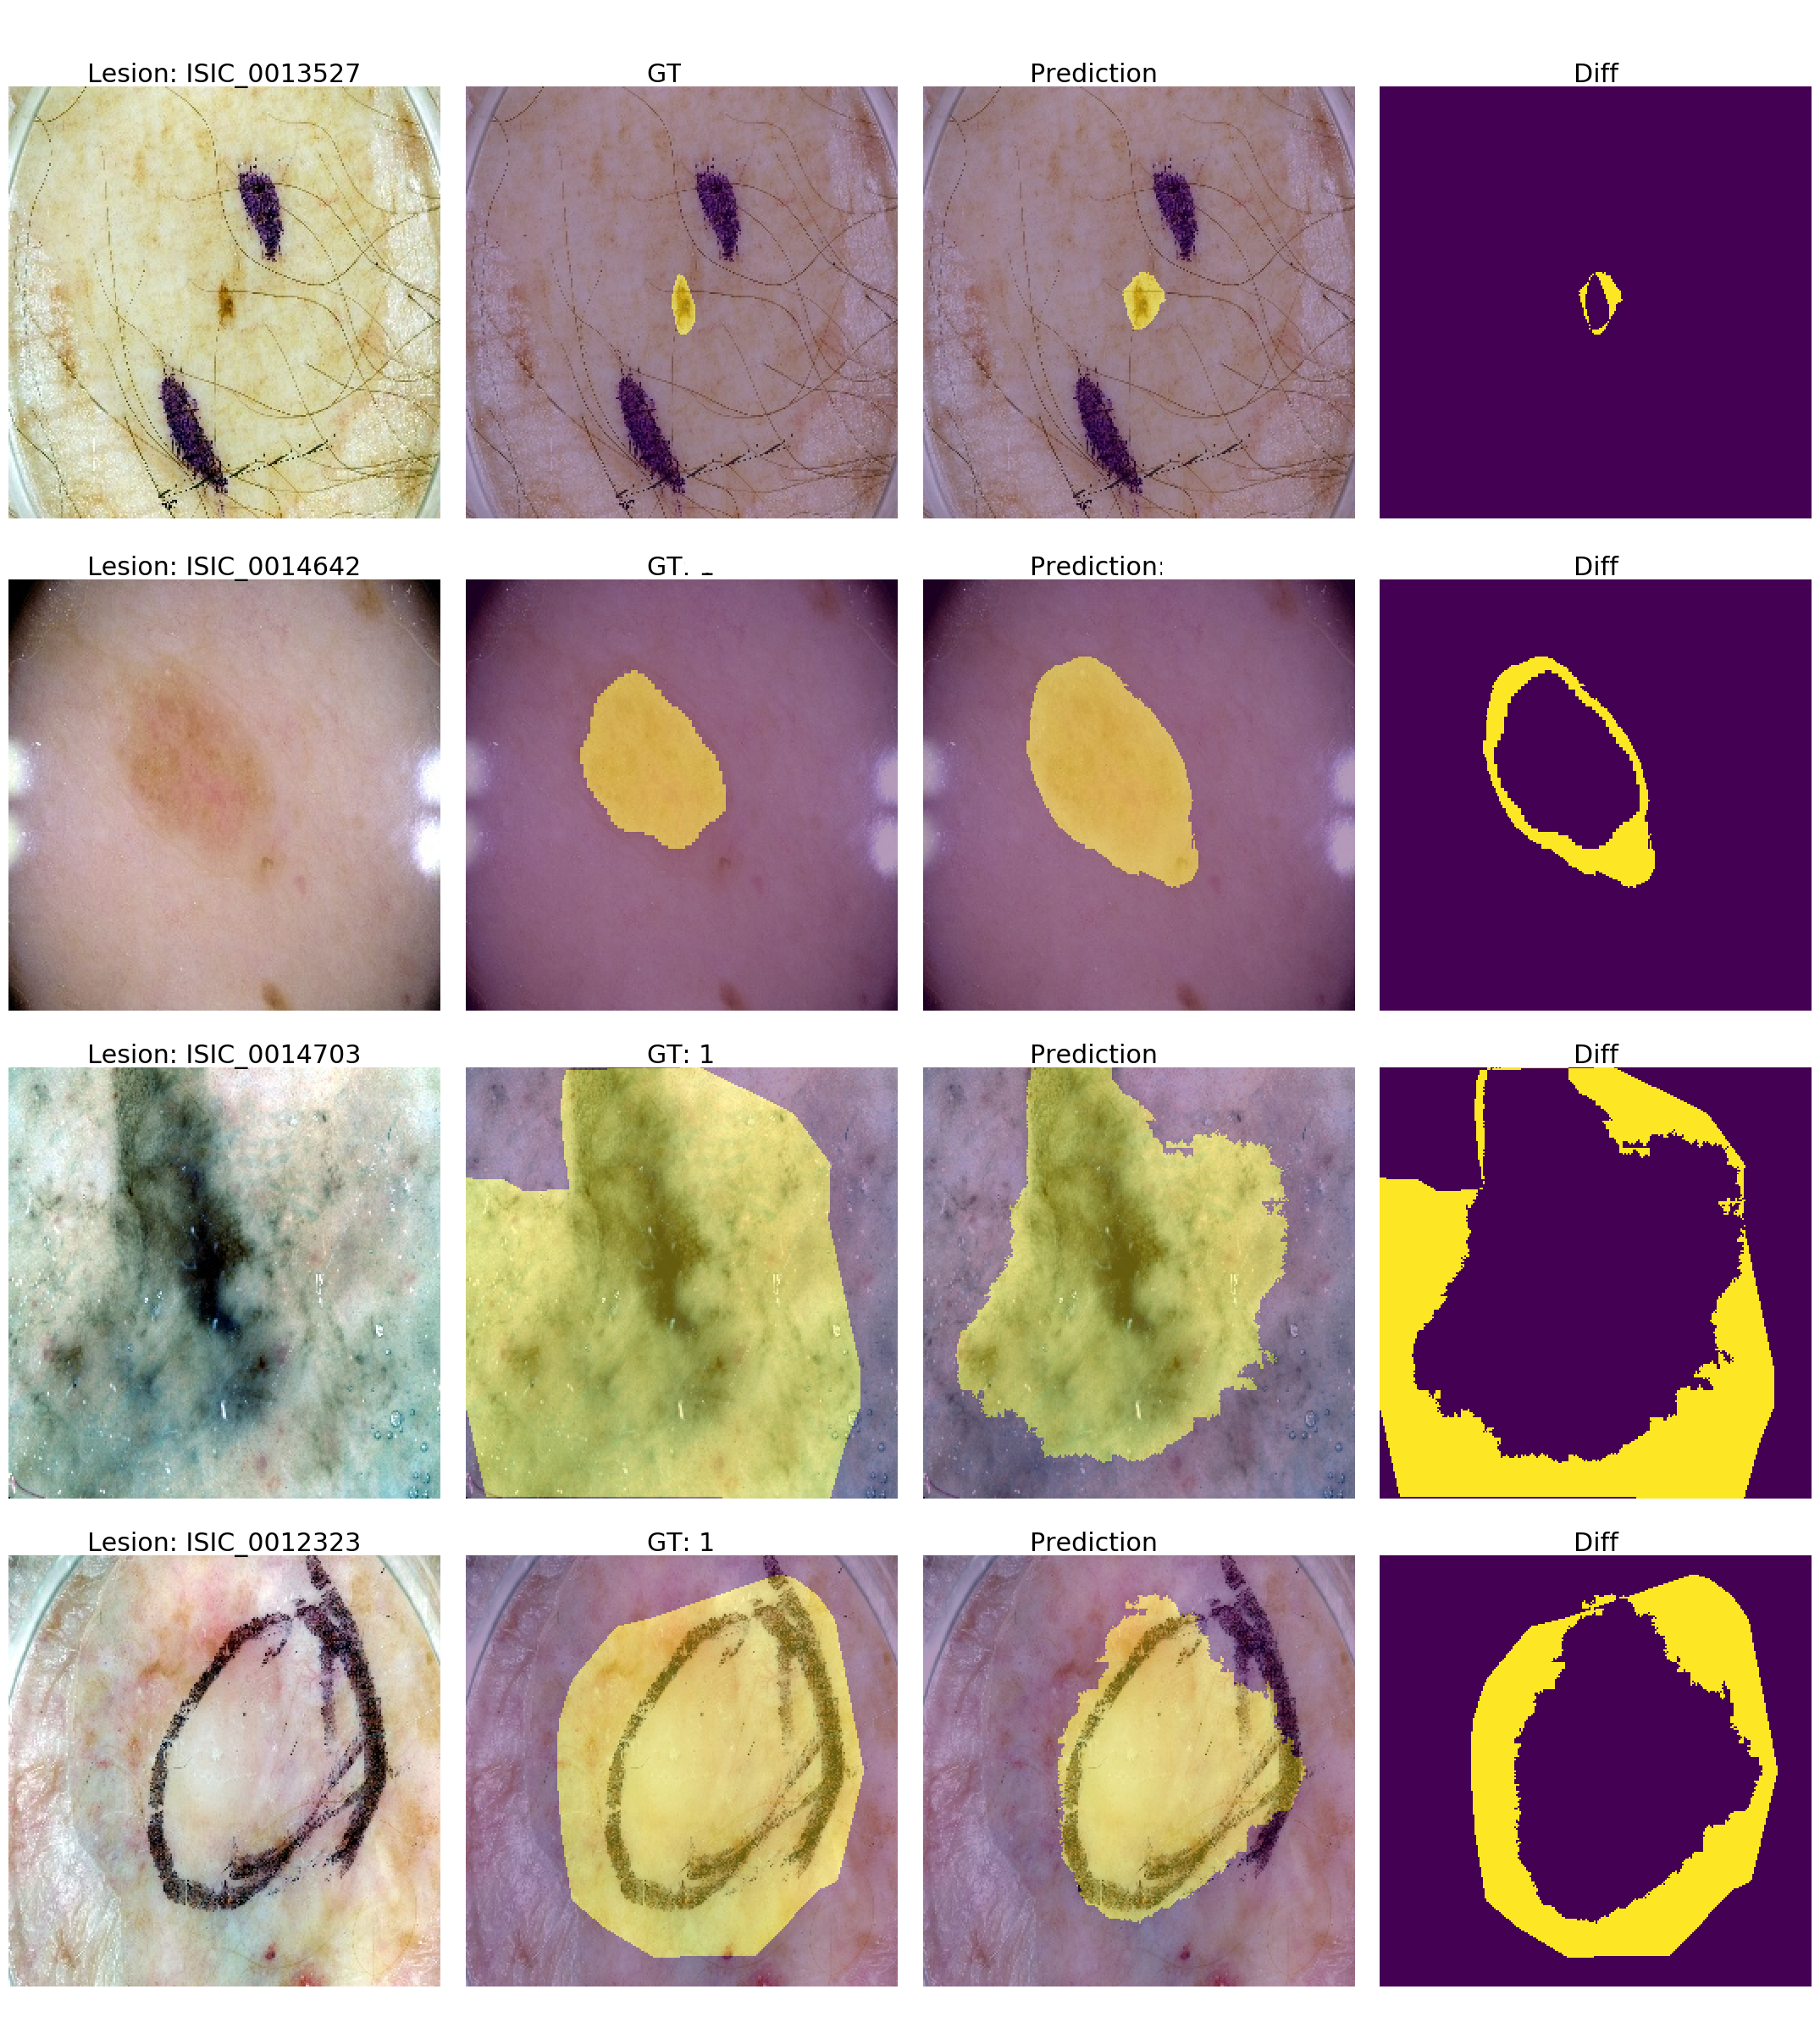
\includegraphics[width=\columnwidth]{bad_results.png}}
\caption{Qualitative assessment of segmentation result}\label{result_samples}
\end{figure}

The best result on our validation set was obtained using the Ensemble strategy.  It achieves a 85.39\% Jaccard index and 78.43\% Threshold Jaccard index (with cut at 65\%). Surprisingly, it did not score so well with the online score and given official validation set, scoring 71.4\%.  The small size of the official validation set and the threshold at 65\% may be the reason for that (one change in prediction from 64\% or 66\% Jaccard makes a huge difference in the average threshold jaccard index). The BestDice strategy achieved an online score of 75.5\% with the official validation set.   Anyway, the top ranked participant in 2017 achieved an average Jaccard Index of 76.5\%, which should be compared with our 85.39\% score.

Visually the best segmentations are almost indentical to the ground truth (see Figure \ref{good}). But we can learn even more from our mistakes. Analysing the worse segmentations there are cases where as non specialists is hard to say if the algorithm was wrong or the ground truth was; there are cases where our algorithm got confused by the pen marker or the glass used by the doctor; and it is clear that in general it doesn't do a good job when the lesion is small relative to the overall image. 

\section{Lesion Classification}
\label{classification}

\subsection{Classification Model}
We used Resnet50, an architecture which has been very succesful in image classification problems. We tried using Resnet101 and Resnext101, but due to the lack of computer resources they didn't suit the fast iteration process our research needed. We used the fastai implementation of Resnet50, which has some improvements over the original model proposed by \cite{resnet}. We customized the Resnet50 model pretrained with the Imagenet dataset~\cite{imagenet}, by first, removing all the steps from the adaptive pooling onwards keeping only Resnet backbone as a feature extractor. Then we plugged a very simple network consisting of:
\begin{itemize}
\item BatchNorm1d (1024, momentum=0.1)
\item Dropout (p=0.25)
\item Linear (input=1024, output=512)
\item ReLU 
\item BatchNorm1d (1024, eps=1e-5, momentum=0.1)
\item Dropout (p=0.5)
\item Linear (input=512, output=7)
\item LogSoftmax
\end{itemize}
We used Adam optimizer and the negative log likelihood loss function.

\subsection{Data and Augmentation}
We used “ISIC 2018: Skin Lesion Analysis Towards Melanoma Detection” grand challenge datasets \cite{codella, ham}. When we used a pretrained Task1 model, we considered that external data was used. All images were first resized to 224x224 and a color balance copy of the dataset was made. Random transformations on input images to agument the dataset were made: dihedral transformation, rotation (up to 35 degrees), zooming (up to 1.05), fliping and random lightining changes. The official training dataset was then splited in 3-folds of training and validation datasets.  


\subsection{Classification: Experiments and Training}
\begin{figure}[htbp]
\centerline{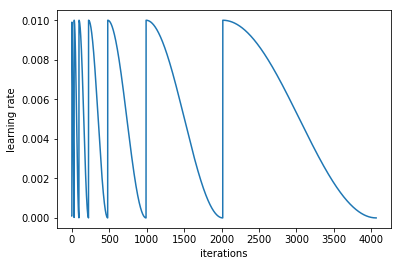
\includegraphics[width=.8\columnwidth]{cycle.png}}
\caption{Cosine cosine annealing learning rate strategy.}
\label{fig}
\end{figure}

% \begin{figure}
% \centering
% \subfloat[Learning Rate Optimization]{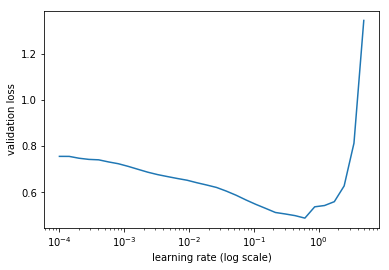
\includegraphics[width=.5\columnwidth]{LR_find.png}}
% \subfloat[cyclical learning rate policy]{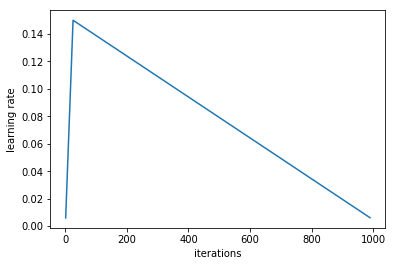
\includegraphics[width=.5\columnwidth]{lr_cycle.png}}\hfil
% \subfloat[superconvergence]{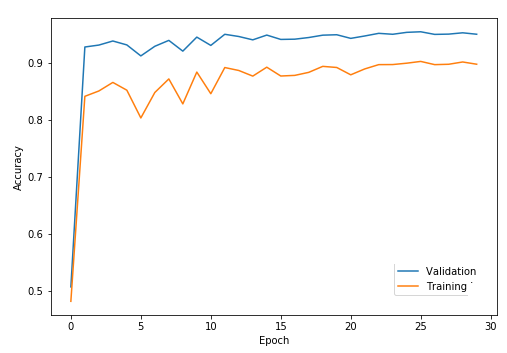
\includegraphics[width=\columnwidth]{accuracy_epoch.png}}
% \caption{colocar aqui}\label{lr_find_chart}
% \end{figure}

Priliminar results showed that the color balanced dataset was performing worse than the original and we kept the later. The training procedure was similar to Task 1 (\ref{sec:seg_training}), but we used a cosine annealing learning rate strategy (see figure \ref{cosine}) instead of the one cycle policy (both proposed by \cite{leslie}). We then tried 3 strategies:

\emph{SnapEsem}: We saved snapshots of our model during training and then made an ensemble of those snapshots, as proposed by \cite{snapshots}.

\emph{CropBest}: We applied our segmentation algorithm from Task1 to the dataset of Task3, croping the images by the lesion mininum bounding rectangle. We used a pretrained model from SnapEsem and retrained it using the croped images.

\emph{KFoldCrop}: We repeated CropBest strategy to 3 different folds and ensemble them. 

On all strategies we applied Test Time Augmentation (TTA) with 5 augmentations per input to improve results.

\subsection{Classification Results}

% Please add the following required packages to your document preamble:
% \usepackage{booktabs}
\begin{table}[]
\centering
\caption{Classification Results.}
\label{tabela}
\begin{tabular}{@{}rrr@{}}
\toprule
            & \multicolumn{1}{c}{Accuracy (\%)} & \multicolumn{1}{c}{Online Score} \\ \midrule
SnapEsem & \(89.71\)& \(84.6\)                                  \\ \midrule
CropBest   & \(93.26\)&  \(76.4\)                                \\ \midrule
KfoldCrop    & \(92.31\)  & \(75.4\)                              \\ \bottomrule
\end{tabular}
\end{table}

Although the best result within our validation set was obtained using the CropBest strategy, we believe that the KfoldCrop can be more general. Interesting to point that all strategies had better accuracy than dermatologists which have an accuracy of 75\% to 84\%\cite{isic}. 

Better than dermatologist specialists (diagnostic accuracy of 75\%-84\%).

\section{Computational Resources\label{resources}}
We used Paperspace GPU Cloud service for running all our experiments. The instance server had: 8 cores CPU with 30GB of RAM, Quadro P4000 8 core GPU with 8GB of RAM. 
The code was developed in PyTorch and Fast.ai\cite{fastai} on Jupyter Notebooks.
\section{Conclusion and Future Work}

This paper descibes our approach for the ISIC Challenge 2018. For the Lesion Segmentation Task, our model Unet34 achieves 77.5\% in the competition threshold jaccard index, which is better than previous results in the competition. For the Lesion Classification, we developed an ensemble strategy that achieves an online score of 84.6\%, which is on the upper bound of dermatologists accuracy range.

Future work could improve in many ways. For lesion segmentation, we could repeat the experiment using other architectures as feature extractors. Test time augmentation could be applied, it made difference in our classification algorithm and was not implemented due to the difficulties of inversing the augmentations to later average.  We suggest to implement a preprocessing pipeline for removing the pen marks in images and maybe a 2 step process can be developed to roughly finding where the lesion is and croping a part of the input image to prevent the bad results due to lesion size. For lesion classification, one could different resnet variations as backbone (resnet18, resnet101, resnext101, etc) and/or using inception. We didn't have time to use the snapshots of the croped images and just used the final model in the kfold, and this may show better results.


\selectlanguage{english}
\bibliographystyle{IEEEtran}
\bibliography{references}

\end{document}
